When the geometry is created, the problem can be defined. \\\\
%In the top menu bar click: Data-> Problem Data and alter the variables to your liking, for explanation of the variables, see Section @@@. 

\subsection{Materials}
todo
%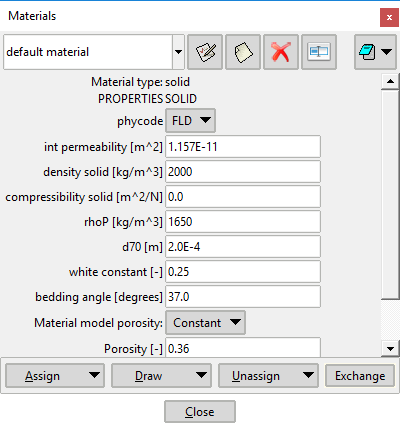
\includegraphics{materialsWindow.png}
%\begin{enumerate}
%	\setlength\itemsep{2mm}
%	\item In the top menu bar click:  Data-> Materials
%	\item In the Materials window click on Rename Materials 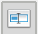
\includegraphics{rename.png} to rename the material from “default material”  
%	\item In the Materials window enter all the material properties, see section @@ for explanation on the variables
%	\item In the Materials window, when all properties are filled. Assign the the material to either Line, Surfaces or Volumes in the geometry view.
%	\item In the Materials window, in order to add a new material, click on New material 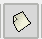
\includegraphics{newMaterial.png} and repeat the aforementioned steps
%	\item In the Materials window, the materials can be unassigned by clicking on Unassign and select the lines,surfaces or volumes in the geometry view.
%	\item In the Materials window, the materials are shown by clicking on Draw
%	
%	\item Materials can be exported or imported to/from other GID projects.In the Materials window, click on exchange and select the *.mat file from another project. In the new "Exhange Materials" window, move the materials to your liking and click on apply or save. Reopen de materials window to see your changes.
%\end{enumerate}

\subsection{Boundary conditions}
todo 
%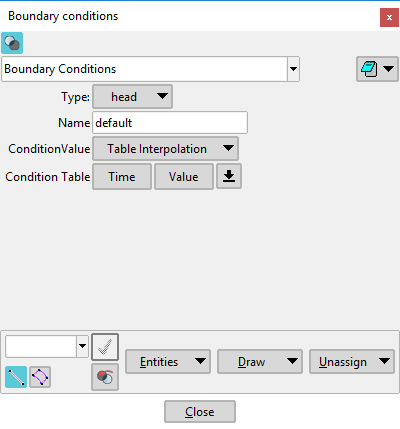
\includegraphics{boundaryConditionsWindow.png}
\begin{enumerate}
		\setlength\itemsep{2mm}
%	\item In the top menu bar click: Data-> Conditions->Boundary conditions 
%	\item In the Boundary conditions window, choose the type of boundary (head, flux, pressure, seepage, general).
%	\item In the Boundary conditions window, fill in the name of your condition
%	\item In the condition table, fill in the boundary condition values (flux or head, depending on the condition type) and the corresponding timesteps. It is also possible to copy the boundary condition values and timesteps from excel. Note that the boundary condition is constant from the last filled in time step.
	\item Before the boundary conditions can be assigned to the geometry, it is important to understand the following box:\\	
	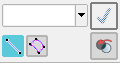
\includegraphics{assignBoundaryConditionBox.png}
	\begin{itemize}
		\item Use the text box to fill in the identifier of the condition (for example the condition name) or select an existing boundary condition
		\item Click on  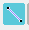
\includegraphics{assignToLine.png} to assign the boundary condition to lines, click on 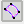
\includegraphics{assignToSurface.png}  to assign the boundary condition to surfaces.
		\item  Click on 
\includegraphics{acceptChange.png}  to assign the filled in boundary condition values to an existing boundary condition which is selected in the text box.
		\item Click on 
\includegraphics{createNewGroup}  to create a new group and assign the group to the geometry (lines or surfaces, depending which option is chosen)
	\end{itemize}
%	\item When a boundary condition is assigned to the geometry, a new group is created. The groups are shown in the layers and group window in the groups tab. When the layers and group window is not shown: on the Standard Gid Toolbar, click on the layers button 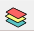
\includegraphics{layersButton} 
%	\item To assign an existing boundary condition to another line/surface, in the groups window, select your group and click on "assign the selected entity to a group" 
\includegraphics{createNewGroup.png}. Now click on either lines or surfaces and assign your boundary condition to the lines or surfaces in the geometry view. 
%	\item To unassign an existing boundary condition, in the groups window, select your group and click on "unassign the selected entity from a group" 
\includegraphics{unassignGroup.png}. Now click on either lines or surfaces and unassign your boundary condition from the lines or surfaces in the geometry view. 	
\end{enumerate}

\subsection{Structural elements and interfaces}
\begin{enumerate}
	\item To create a structural element, on the top menu bar click on \textit{GeoMechanicsApplication => elements}. 
	\item From the \textit{Elements} window which appeared, from the top drop-down menu. Select the preferred structural element (Beam, Shell thin corotational, Shell thick corotational, Truss or Cable). The structural element can then be assigned to the geometry.
	\item In order to create an interface between the soil and the structural element. Multiple GiD-layers need to be created in GiD. One layer needs to be the layer of the structural elements, the next layer is the soil on one side of the structural element, the next layer being the soil on the other side of the structural element.
	 
	
	
\end{enumerate}

